\documentclass[12pt, a4paper]{article}
\usepackage[utf8]{inputenc}
\usepackage[spanish]{babel}
\usepackage[table]{xcolor}
\usepackage{url, hyperref}
\usepackage{graphicx, listings, xcolor, adjustbox, caption, subcaption, float, amsmath}

\definecolor{codegreen}{rgb}{0,0.6,0}
\definecolor{codegray}{rgb}{0.5,0.5,0.5}
\definecolor{codepurple}{rgb}{0.58,0,0.82}
\definecolor{backcolour}{rgb}{0.95,0.95,0.92}

\lstdefinestyle{mystyle}{
    backgroundcolor=\color{backcolour},   
    commentstyle=\color{codegreen},
    keywordstyle=\color{magenta},
    numberstyle=\tiny\color{codegray},
    stringstyle=\color{codepurple},
    basicstyle=\ttfamily\footnotesize,
    breakatwhitespace=false,         
    breaklines=true,                 
    captionpos=b,                    
    keepspaces=true,                 
    numbers=left,                    
    numbersep=5pt,                  
    showspaces=false,                
    showstringspaces=false,
    showtabs=false,                  
    tabsize=2
}

\setlength{\parindent}{0pt}
\setlength{\parskip}{12pt}
\renewcommand{\arraystretch}{1.5}
\lstset{style=mystyle, language=Octave}

\title{\vspace{-3cm}Tarea 4: Recorrido de ciudades con ACO}
\author{
    Universidad Autónoma de San Luis Potosí\\ 
    Facultad de Ingeniería - Ing. en Sistemas Inteligentes\\ 
    \textbf{Materia:} Cómputo Bioinspirado \\
    \textbf{Prof:} Dr. Cesar Augusto Puente Montejano  \\
    \textbf{Autor:} Angel de Jesús Maldonado Juárez
}
\date{\textbf{Fecha de entrega:} miércoles 7 de septiembre de 2022}

\begin{document}

\maketitle

\begin{center}
    \rule{\textwidth}{0.5pt}
    \begin{abstract}
        \noindent El algoritmo \emph{Optimización por Colonia de Hormigas} es un tipo de algoritmo de \emph{Inteligencia de Enjambre} que está basado en el comportamiento de las hormigas que tienen cuando buscan una fuente de alimentos para su colonia. El principal mecanismo que tienen para lograr su objetivo es la comunicación entre hormigas mediante feromonas. Este artículo trata a detalle este mecanismo y cómo puede utilizarse esta analogía para resolver el problema \emph{Traveling Sales Person Man}, junto con la ejecución del algoritmo con distintos parámetros para ver cómo afectan los mismos en el rendimiento final.
    \end{abstract}
    \rule{\textwidth}{0.5pt}
\end{center}

\section{Inteligencia de Enjambre}\label{title1}
La \emph{Inteligencia de Enjambre} es un comportamiento presente en seres vivos que suelen actuar en grupo, la idea principal de este comportamiento es que existen individuos (\emph{agentes}) que forman parte de una población, y por si solos muestran una conducta bastante simple, pero cuando se observa a toda una población de individuos en conjunto, pareciera que hay coordinación y comunicación entre todos para lograr un común objetivo. Por ejemplo, una paloma por si sola vuela hacia cualquier dirección y en cualquier momento, pero cuando varias palomas vuelan en conjunto pareciera que alguien las estuviera guiando para ir hacia la misma dirección en el mismo momento. A este comportamiento presente específicamente en los pájaros se le conoce como \emph{bandada}.

\section{Optimización por Colonia de Hormigas}
El algoritmo \emph{Optimización por Colonia de Hormigas} (Ant Colony Optimization - ACO) utiliza como inspiración el comportamiento de las hormigas en conjunto cuando buscan una fuente de alimento. Una sola hormiga en este contexto tiene 3 simples pasos para lograr su objetivo: caminar en busca de alimento, encontrar una fuente de alimento, y volver al hormiguero dejando un rastro de feromonas por el camino que siguió para encontrar la fuente de alimento. Este último paso es clave cuando se analiza a todo un conjunto de hormigas, ya que, la principal forma de comunicación de las hormigas es mediante estas feromonas; cuando una hormiga percibe un rastro de feromonas sigue la misma ruta que dejó la otra hormiga cuando regresó al hormiguero después de encontrar una fuente de alimento, y al mismo tiempo también deja su propia carga de feromonas, aumentando la probabilidad de que otras hormigas sigan esa misma ruta a la fuente de alimento.

Esta analogía puede utilizarse para resolver una gran variedad de problemas de búsqueda, este reporte se enfoca en el problema \href{https://en.wikipedia.org/wiki/Travelling_salesman_problem}{\emph{Travelling Sales Person}} (TSP), el planteamiento es el siguiente: \emph{"Dada una lista de ciudades y las distancias entre cada para de ciudades, ¿cuál es la ruta más corta en la que se puede visitar cada ciudad exactamente una vez y regresar al punto de partida?"}. Para poder resolver el problema, el espacio que las hormigas deben explorar puede representarse mediante una \textbf{matriz de costos} $D$ (distancias). Otra información que se necesita en el espacio es el nivel de feromonas que hay en cada posible ruta, para ello también se puede representar mediante una \textbf{matriz de feromonas} $\tau$. Finalmente, las hormigas son las \emph{entidades} encargadas de explorar el espacio del problema, para ello cada una tiene que realizar las acciones que describen su comportamiento natural: seleccionar una ruta con base en el rastro de feromonas que ya existe y dejar su propio rastro de feromonas hasta llegar a la fuente de alimento (solución del problema). La \textbf{actualización de feromonas} en el espacio del problema puede representarse de la siguiente manera:

\begin{equation} \label{eq:1}
    \tau_{i,j}^k=\sum_{k=1}^m\Delta\tau_{i,j}^k
\end{equation}

Donde:

$\tau_{i,j}^k$ es el nivel de feromonas en la arista $i,j$ colocado por la hormiga $k$.

$\sum_{k=1}^m\Delta\tau_{i,j}^k$ es la sumatoria del nivel de feromonas que las demas hormigas depositaron.

$Delta\tau_{i,j}^k$ es la cantidad de feromonas que la hormiga $k$ decide poner sobre la arista $i,j$; $\frac{1}{L_k}$ ($L$ es el costo de la arista) si decide visitar la arista, y $0$ si no la visitará.

Existe otra versión de la ecuación para el nivel de feromonas (\ref{eq:1}) en el cual introduce el componente de \textbf{evaporización} para que las hormigas futuras no vayan por caminos poco ideales:

\begin{equation}
    \tau_{i,j}^k=(1-p)\tau_{i,j}\sum_{k=1}^m\Delta\tau_{i,j}^k
\end{equation}

Donde $p<1$ es una constante que indica la magnitud de la evaporización.

La \textbf{elección del camino} de las hormigas puede representarse utilizando probabilidades, combinando tanto la matriz de costos $D$ y la matriz de feromonas $\tau$:

\begin{equation}
    P_{i,j}=\frac{(\tau_{i,j})^\alpha(\eta_{i,j})^\alpha}{\sum((\tau_{i,j})^\alpha(\eta_{i,j})^\alpha)}
\end{equation}

Donde:

$\eta_{i,j}$ representa la calidad de la arista $i,j$ ($\eta_{i,j}=\frac{1}{L_{i,j}}$).

$\alpha,\beta$ determina el impacto de $\tau$ o $\eta$.

$\sum((\tau_{i,j})^\alpha(\eta_{i,j})^\alpha)$ es la sumatoria del nivel de feromonas y la calidad de todas las aristas que una hormiga tiene para elegir.

Con estas tres ecuaciones puede generarse un algoritmo para resolver el problema TSP basado en Colonias de Hormigas.

\section{Problema TSP con ACO}
El programa y algoritmo completo que se utiliza en este reporte fue implementado por S. Mostapha Kalami Heris \cite{AntColon50:online}. Este código tiene la función \lstinline{CreateModel()} en la que genera un vector de coordenadas \lstinline{x}, otro vector para las coordenadas \lstinline{y} correspondientes, la matriz de costos \lstinline{D}, y un número \lstinline{n} que representa la cantidad de nodos/ciudades que visitarán las hormigas, que en este caso puede calcularse contando el número de elementos del vector \lstinline{x} o \lstinline{y}. El código por defecto tiene una definición específica para todas estas variables, pero se modificó de forma que pudiera leer un \emph{archivo de coordenadas} (\lstinline{.txt}) y otro \emph{archivo de matriz} (\lstinline{.txt}) para generalizar el problema (\lstinline{CreateModelFromFile.m}):

\lstinputlisting{src/CreateModelFromFile.m}

Con esta modificación el resto del código funciona correctamente, incluyendo la visualización del tour de las hormigas y la gráfica final de la historia de las iteraciones. El establecimiento de los parámetros para la ejecución del algoritmo se define en el archivo \lstinline{aco.m}:

\lstinputlisting{src/aco.m}

En este mismo archivo se reemplaza la invocación de la función \lstinline{CreateModel()} por \lstinline{CreateModelFromFile(filename)} para generar el modelo utilizando una matriz de costos y vectores de coordenadas utilizando archivos \lstinline{.txt}.

Para los experimentos se utilizan algunos de los \emph{datasets} de \textbf{CITIES} \cite{CITIESCi13:online}, en específico \emph{UK12}, \emph{WG59}, y \emph{SP11}. A continuación se meustran los resultados para cada uno de estos \emph{datasets} con distinta configuración de parámetros.

\subsection{UK12}

\begin{table}[!ht]
    \begin{adjustbox}{width=\textwidth}
        \begin{tabular}{|c|c|c|c|c|c|c|}
            \rowcolor{yellow}
            \hline
            $MaxIt$ & $nAnt$ & $alpha$ & $beta$ & $rho$ & Iteración del resultado & $BestCost$ \\
            \hline
            $50$    & $10$   & $1$     & $0.5$  & $0.1$ & $46$                    & $1820$     \\
            \hline
            $50$    & $10$   & $1$     & $0.7$  & $0.1$ & $34$                    & $1814$     \\
            \hline
            $50$    & $10$   & $1$     & $1$    & $0.1$ & $41$                    & $1733$     \\
            \hline
            $30$    & $30$   & $1$     & $1$    & $0.3$ & $18$                    & $1733$     \\
            \hline
            $20$    & $35$   & $1$     & $1$    & $0.5$ & $8$                     & $1733$     \\
            \hline
        \end{tabular}
    \end{adjustbox}
\end{table}

\textbf{Peor resultado vs. Mejor resultado}:

\begin{figure}[H]
    \centering
    \begin{subfigure}[b]{0.45\textwidth}
        \centering
        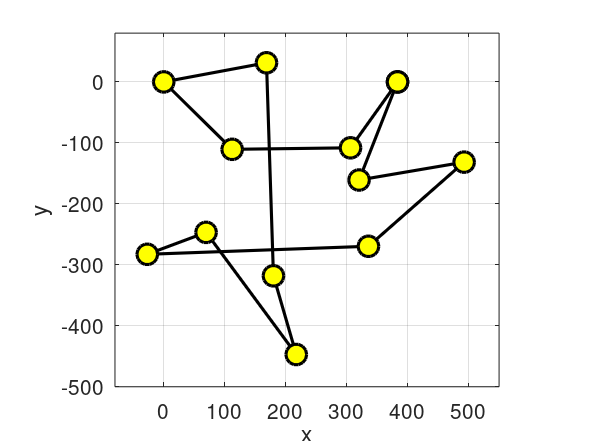
\includegraphics[width=\textwidth]{img/uk12-worst-graph.png}
        \caption{Grafo peor resultado}
        \label{fig:uk12-worst-graph}
    \end{subfigure}
    \hfill
    \begin{subfigure}[b]{0.45\textwidth}
        \centering
        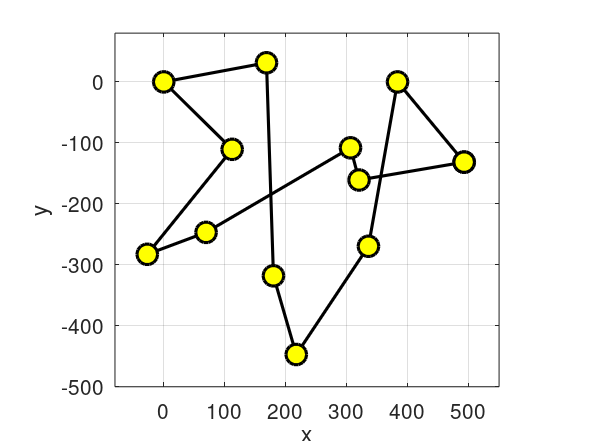
\includegraphics[width=\textwidth]{img/uk12-best-graph.png}
        \caption{Grafo mejor resultado}
        \label{fig:uk12-best-graph}
    \end{subfigure}
    \caption{Grafos UK12}
    \label{fig:uk12-graphs}
\end{figure}

\begin{figure}[H]
    \centering
    \begin{subfigure}[b]{0.45\textwidth}
        \centering
        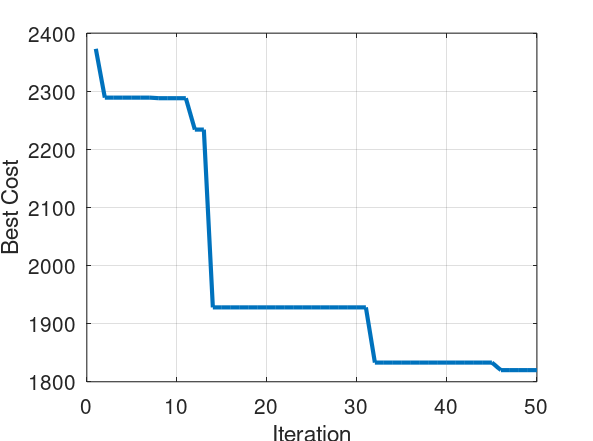
\includegraphics[width=\textwidth]{img/uk12-worst-history.png}
        \caption{Historia peor resultado}
        \label{fig:uk12-worst-history}
    \end{subfigure}
    \hfill
    \begin{subfigure}[b]{0.45\textwidth}
        \centering
        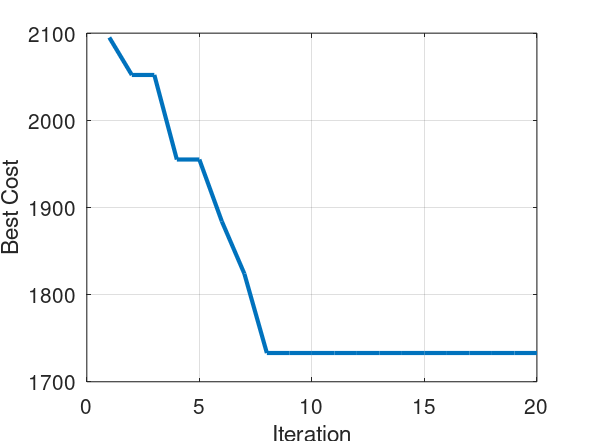
\includegraphics[width=\textwidth]{img/uk12-best-history.png}
        \caption{Historia mejor resultado}
        \label{fig:uk12-best-history}
    \end{subfigure}
    \caption{Historias UK12}
    \label{fig:uk12-histories}
\end{figure}

\subsection{GW59} \label{subsec:gw59}

\begin{table}[!ht]
    \begin{adjustbox}{width=\textwidth}
        \begin{tabular}{|c|c|c|c|c|c|c|}
            \rowcolor{yellow}
            \hline
            $MaxIt$ & $nAnt$ & $alpha$ & $beta$ & $rho$   & Iteración del resultado & $BestCost$ \\
            \hline
            $20$    & $20$   & $1$     & $1$    & $0.05$  & $18$                    & $1952$     \\
            \hline
            $20$    & $40$   & $1$     & $1$    & $0.2$   & $18$                    & $1397$     \\
            \hline
            $100$   & $60$   & $1$     & $1$    & $0.3$   & $93$                    & $1105$     \\
            \hline
            $100$   & $70$   & $1$     & $1$    & $0.5$   & $88$                    & $1104$     \\
            \hline
            $100$   & $60$   & $1$     & $1$    & $0.6$   & $78$                    & $1100$     \\
            \hline
            $130$   & $60$   & $1$     & $1$    & $0.5$   & $120$                   & $1091$     \\
            \hline
            $210$   & $60$   & $1$     & $1$    & $0.53$  & $157$                   & $1064$     \\
            \hline
            $300$   & $60$   & $1$     & $1$    & $0.534$ & $253$                   & $1061$     \\
            \hline
        \end{tabular}
    \end{adjustbox}
\end{table}

\textbf{Peor resultado vs. Mejor resultado}:

\begin{figure}[H]
    \centering
    \begin{subfigure}[b]{0.45\textwidth}
        \centering
        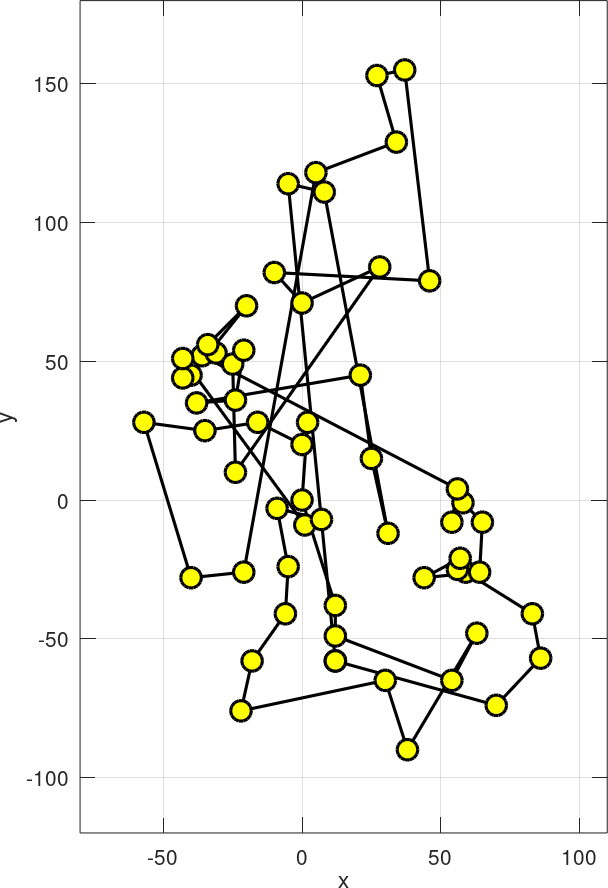
\includegraphics[width=0.6\textwidth]{img/gw59-worst-graph.png}
        \caption{Grafo peor resultado}
        \label{fig:gw59-worst-graph}
    \end{subfigure}
    \hfill
    \begin{subfigure}[b]{0.45\textwidth}
        \centering
        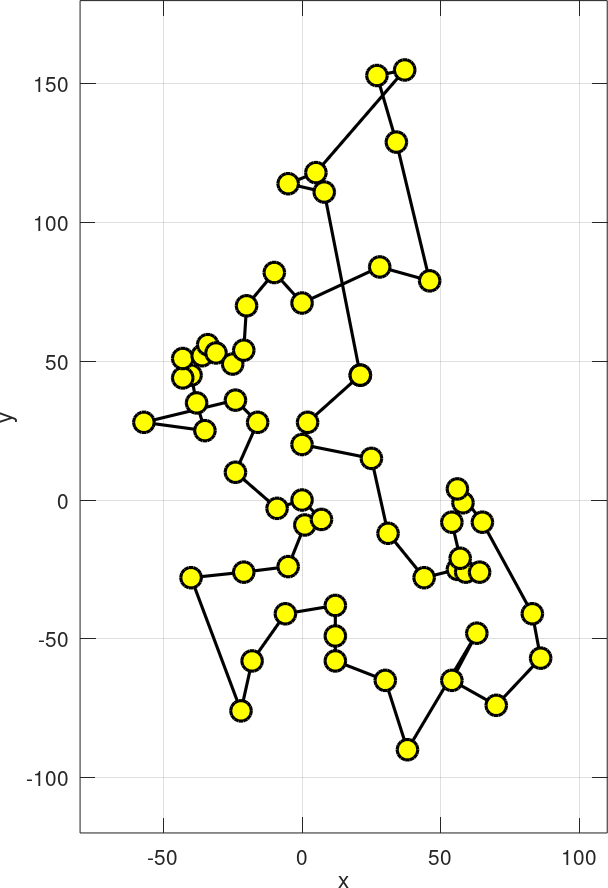
\includegraphics[width=0.6\textwidth]{img/gw59-best-graph.png}
        \caption{Grafo mejor resultado}
        \label{fig:gw59-best-graph}
    \end{subfigure}
    \caption{Grafos gw59}
    \label{fig:gw59-graphs}
\end{figure}

\begin{figure}[H]
    \centering
    \begin{subfigure}[b]{0.45\textwidth}
        \centering
        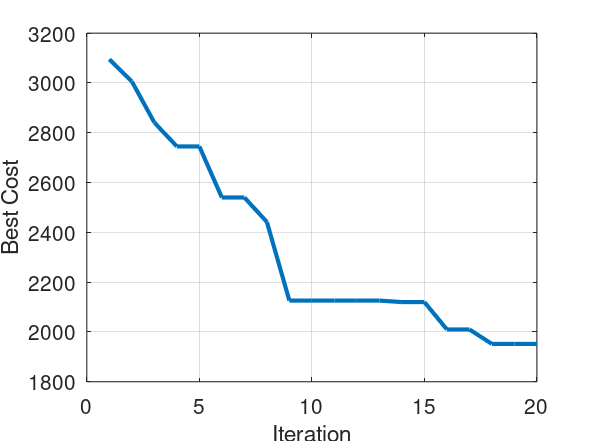
\includegraphics[width=\textwidth]{img/gw59-worst-history.png}
        \caption{Historia peor resultado}
        \label{fig:gw59-worst-history}
    \end{subfigure}
    \hfill
    \begin{subfigure}[b]{0.45\textwidth}
        \centering
        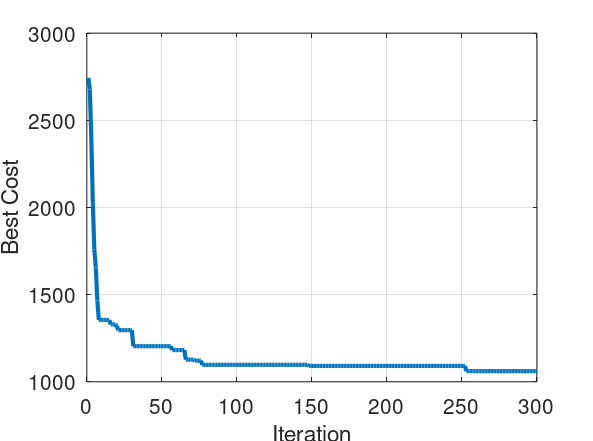
\includegraphics[width=\textwidth]{img/gw59-best-history.png}
        \caption{Historia mejor resultado}
        \label{fig:gw59-best-history}
    \end{subfigure}
    \caption{Historias gw59}
    \label{fig:gw59-histories}
\end{figure}

\subsection{SP11} \label{subsec:sp11}

\begin{table}[!ht]
    \begin{adjustbox}{width=\textwidth}
        \begin{tabular}{|c|c|c|c|c|c|c|}
            \rowcolor{yellow}
            \hline
            $MaxIt$ & $nAnt$ & $alpha$ & $beta$ & $rho$  & Iteración del resultado & $BestCost$ \\
            \hline
            $20$    & $3$    & $1$     & $1$    & $0.9$  & $4$                     & $155$      \\
            \hline
            $20$    & $3$    & $1$     & $1$    & $0.5$  & $10$                    & $138$      \\
            \hline
            $60$    & $9$    & $1$     & $1$    & $0.03$ & $49$                    & $136$      \\
            \hline
            $70$    & $10$   & $1$     & $1$    & $0.02$ & $33$                    & $133$      \\
            \hline
        \end{tabular}
    \end{adjustbox}
\end{table}

\textbf{Peor resultado vs. Mejor resultado}:

\begin{figure}[H]
    \centering
    \begin{subfigure}[b]{0.45\textwidth}
        \centering
        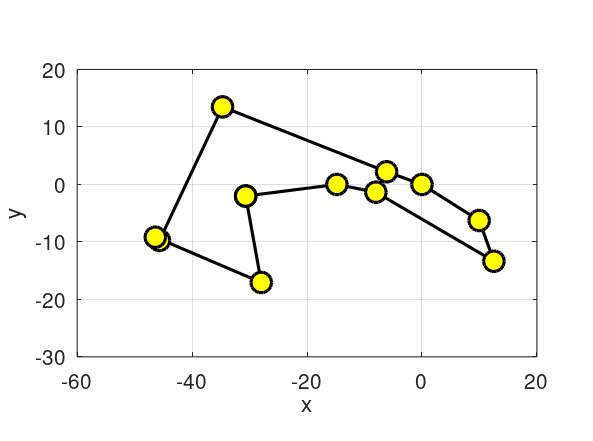
\includegraphics[width=\textwidth]{img/sp11-worst-graph.png}
        \caption{Grafo peor resultado}
        \label{fig:sp11-worst-graph}
    \end{subfigure}
    \hfill
    \begin{subfigure}[b]{0.45\textwidth}
        \centering
        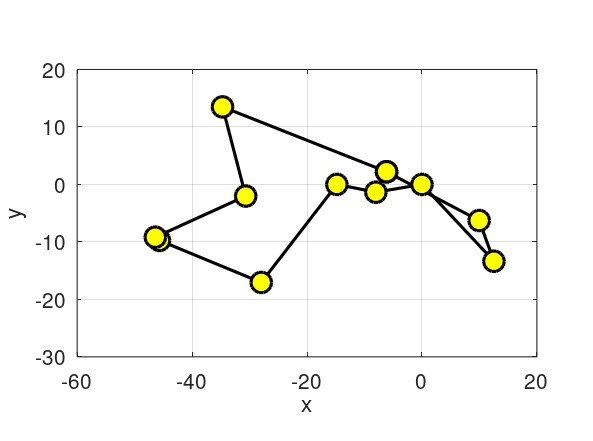
\includegraphics[width=\textwidth]{img/sp11-best-graph.png}
        \caption{Grafo mejor resultado}
        \label{fig:sp11-best-graph}
    \end{subfigure}
    \caption{Grafos sp11}
    \label{fig:sp11-graphs}
\end{figure}

\begin{figure}[H]
    \centering
    \begin{subfigure}[b]{0.45\textwidth}
        \centering
        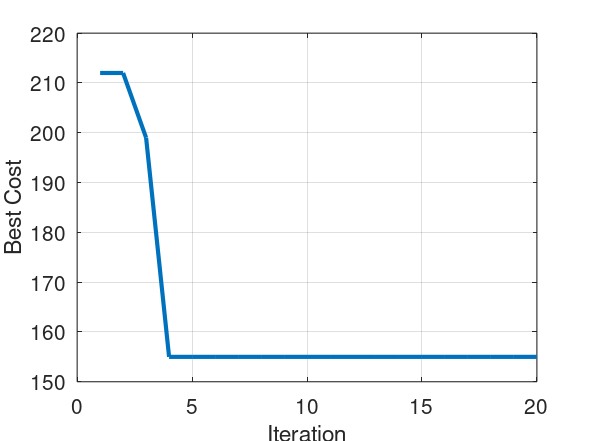
\includegraphics[width=\textwidth]{img/sp11-worst-history.png}
        \caption{Historia peor resultado}
        \label{fig:sp11-worst-history}
    \end{subfigure}
    \hfill
    \begin{subfigure}[b]{0.45\textwidth}
        \centering
        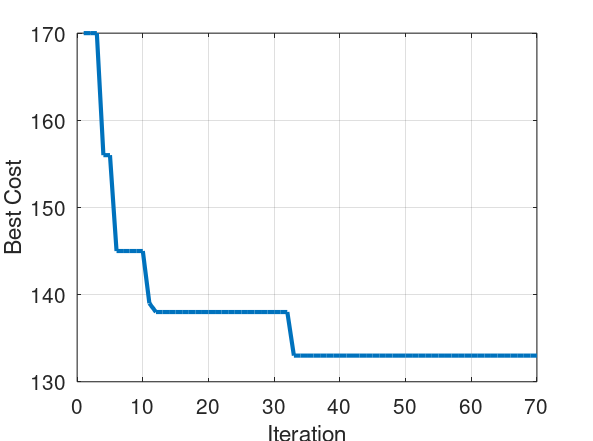
\includegraphics[width=\textwidth]{img/sp11-best-history.png}
        \caption{Historia mejor resultado}
        \label{fig:sp11-best-history}
    \end{subfigure}
    \caption{Historias sp11}
    \label{fig:sp11-histories}
\end{figure}

\section{Conclusiones}
La modificación de los parámetros en el ACO depende mucho del tamaño del espacio del problema; para espacios con muchos lugares por explorar, la \textbf{cantidad de hormigas} (\lstinline{nAnt}) debe ser lo suficientemente grande para que puedan abarcar la mayor cantidad de posibilidades del problema, junto con un \textbf{número de iteraciones} (\lstinline{MaxIt}) suficiente para que les dé tiempo a las hormigas de explorar el espacio. En cambio, si el problema tiene pocos lugares por explorar tanto el \textbf{número de iteraciones} como la \textbf{cantidad de hormigas} no necesitan valores grandes. La modificación de $\alpha$ y $\beta$ impactan bastante en el desempeño de las hormigas, y realmente necesitan estar en balance ambos números para que la decisión de una hormiga para tomar un camino sea neutral ($\alpha=1,\beta=1$). Finalmente, el parámetro $\rho$ (evaporación de las feromonas) tiende a requerir valores muy específicos cuando el espacio de problema es muy grande, como en el caso de la ciudad \href{subsec:gw59}{GW59}, donde $\rho=0.534$. En contraparte, el caso de la ciudad \href{subsec:sp11}{SP11} tuvo que tener un valor de $\rho$ lo suficientemente pequeño para que las pocas hormigas que hay tuvieran suficientes opciones para elegir un camino sin que este desapareciera con el tiempo, además, en un espacio tan pequeño no hace falta que las hormigas descarten caminos porque son pocos los que deberían explorar.

\bibliographystyle{unsrt}
\bibliography{refs}
\nocite{*}

\end{document}
